\documentclass{jsarticle}
\usepackage[dvipdfmx]{graphicx}

\title{楽しい運動計測実習に関するレポート}
\date{\today}
\author{奥屋 直己}

\usepackage[height=26cm,width=16cm]{geometry}

\begin{document}

\maketitle

\section{実験の目的}

この実験の目的は筋肉の活動を筋電センサ、モーションキャプチャを使い計測し、そのデータを解析すると同時に、それぞれの機器の使い方を学ぶことである。

\section{手法}

\subsection{実験}

今実験は腕を水平面内で伸ばす、曲げるの繰り返し運動を動かしやすい速度で動かす時と、それよりも速く動かすときについて、手首、肘、肩の3点の軌道と筋電の波形を計測した。
3点の軌道の計測は、それぞれに反射マーカーをつけ、真上に設置した高速度カメラを使った。
筋電の計測は、上腕二頭筋と上腕三頭筋に筋電計用電極を取り付け、計測した。
それぞれ、サンプリングは200frame/s、1000frame/sとし、同時パルス発生装置を使い、開始時刻を同期した上で20秒間計測した。
この実験では2人の被験者で行った。ただし、1人はデータがうまく取れなかったため、データは実質1人分となった。
\subsection{解析}

今回は筋電センサによる筋電データとモーションキャプチャによる運動軌道データを別々のプログラムで作成する。

\subsubsection{筋電データ}

今回筋電データの解析にはpython3.6.4とC言語を用いた。
まず、筋電データには計測したデータの他にノイズが混ざっていると予測されるため、データの1~40Hzに対してバンドパスフィルタをかけることにより、低周波のノイズを除去した。また、単純にバンドパスフィルタをかけるとデータのピーク位置が実際のデータよりもすこしおそくなってしまう。そのためpythonのfiltfilt関数を使うことにより、順方向と逆方向の両方から1回ずつフィルタをかけ、ズレをなくした。

次にC言語で筋肉の活動度(a(t))を以下の式で評価した。tは時間[s]×$10^3$で求まる。
\begin{equation}
a(t)=\frac{1}{\Delta{T}}\int^{t+\Delta{T}/2}_{t-\Delta{T}/2} |E(t)|
\end{equation}
E(t)は筋電位、幅$\Delta{T}$の窓を200とした。これにより、$\pm0.1$[s]間での筋電位の上昇度を算出することができた。

\subsubsection{運動軌道データ}
運動軌道データの解析用ブログラムの作成にはC言語とシェルスクリプトを用いた。
モーションキャプチャから得たデータはヘッダ部、データ部、テール部が1つのデータとなっているため、ヘッダ部とテール部をinfo-(ファイル名),dat、データ部をpos-(ファイル名).datに分割するシェルスクリプトを作成した。

次に、作成したpos-(ファイル名).datから各関節の各座標データを \textbf{時間,x座標,y座標,z座標} と関節ごとのファイルに抽出するプログラムを作成した。このプログラムでは、サンプリング周波数、マーカー数、ファイル名を引数としており、これらをヘッダ部から抽出し、実行するシェルスクリプトを作成した。さらに、作成したファイルから座標データのみを抽出するシェルスクリプトを作成した。

\section{結果}
モーションキャプチャを使用し、取得した軌道データから以下のグラフを作成した。ただし、動作する腕の真上にカメラを設置したため、本来の動きと左右対称になってしまったため、x軸を逆方向にしている。
\begin{figure}[h]
  \begin{center}
    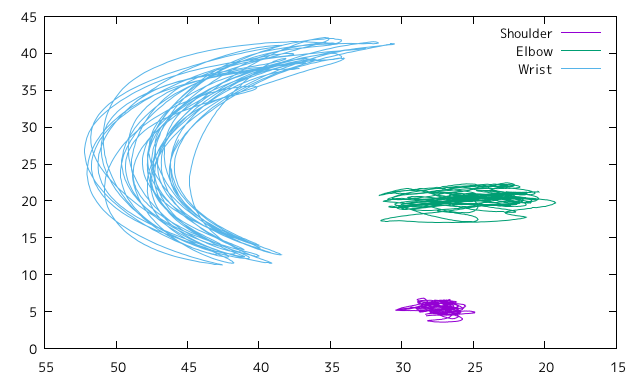
\includegraphics[clip,width=150mm]{Graph_2.png}
    \caption{適切な速さ}
  \end{center}
\end{figure}
\begin{figure}[h]
  \begin{center}
    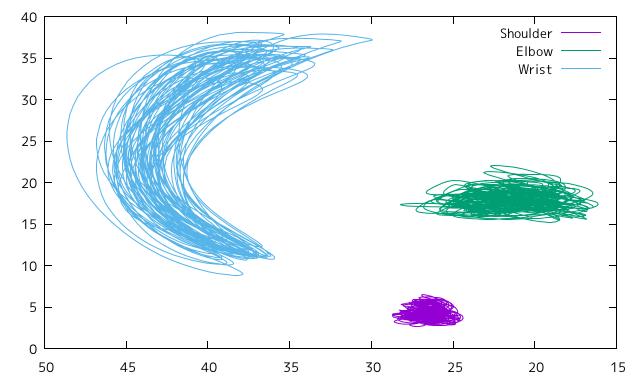
\includegraphics[clip,width=150mm]{Graph_3.png}
    \caption{速い速度}
  \end{center}
\end{figure}

これより、速さでの軌道の違いはほぼないことがわかる。

次にx軸に時間、左のy軸に手首の軌道のy成分(点線)、右のy軸に解析した筋電の大きさ(青線)をとったグラフを示す。
\begin{figure}[h]
  \begin{center}
    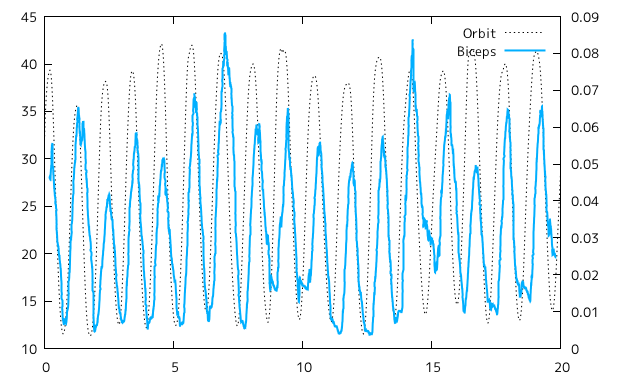
\includegraphics[clip,width=150mm]{Graph_4.png}
    \caption{腕の軌道と筋電の関係}
  \end{center}
\end{figure}

この結果より腕を伸ばしたあと、もう一度腕を曲げる時に、最も筋電位が上昇することがわかる。

次に同じ条件で速く動かした時のグラフを以下に示す。
\begin{figure}[h]
  \begin{center}
    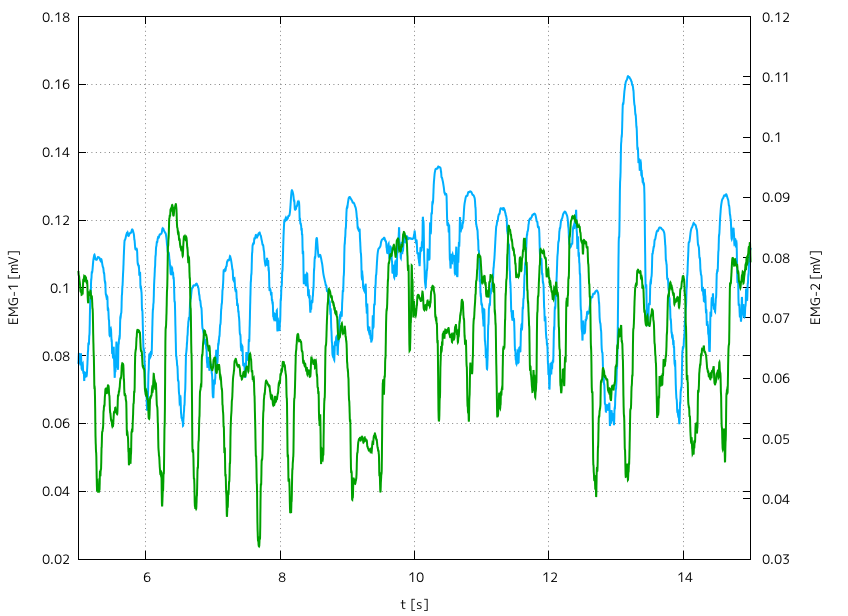
\includegraphics[clip,width=150mm]{Graph_5.png}
    \caption{腕の軌道と筋電の関係(速く動かしたとき)}
  \end{center}
\end{figure}


このままではわかりづらいので、5秒から15秒間の結果を拡大して以下に示す。
\begin{figure}[t]
  \begin{center}
    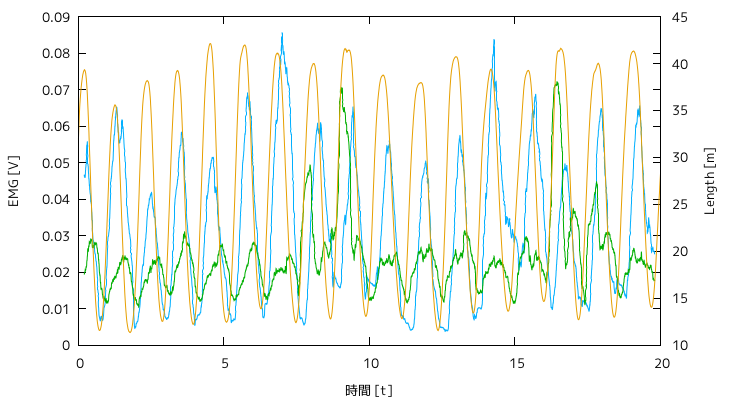
\includegraphics[clip,width=150mm]{Graph_6.png}
    \caption{図4の5秒から15秒}
  \end{center}
\end{figure}
この図からも適切な速度と同様に腕を曲げようとする瞬間に筋電位が上昇することがわかる。

\section{考察}
結果の図3と図5を比べると、両方とも腕を曲げようとするときに筋電位が上昇することがわかった。また、速く動かした場合のほうが筋電位の上昇率が低いことがわかる。ただし、一概に速く動かした場合の方が実際の上昇率が低いとは言えない。今回筋電センサはテープで軽く固定していたため、速く動かした場合の方が筋電センサと皮膚の密着度が低くなったと考えられる。実際に、図4から、速く動かした時の方が、筋電位のブレが大きい。また、図1と図2より、2つの軌道に大きな差はない。このことから、筋電センサをバンドのようなものでしっかりと固定した時も考える必要があると考える。


\end{document}